\documentclass{article}

\usepackage[margin=1in]{geometry}
\usepackage{times}
\usepackage{graphicx}
\usepackage{subcaption}
\graphicspath{{figures/}}
\usepackage{natbib}
\bibliographystyle{plainnat}

\begin{filecontents}{references.bib}
@article{lee2019advanced,
  title={Advanced Subsymbolic Reasoning Mechanisms},
  author={Lee, J. and Park, A.},
  journal={Journal of AI Research},
  volume={64},
  pages={201--220},
  year={2019}
}

@inproceedings{smith2022pitfalls,
  title={Pitfalls of Symbolic Proxies in Real-World AI},
  author={Smith, T. and Jordan, M.},
  booktitle={ICLR},
  year={2022}
}

@inproceedings{clark2020assessing,
  title={Assessing The Reliability of Deep Relational Reasoning},
  author={Clark, K. and Brown, S.},
  booktitle={NeurIPS},
  year={2020}
}
\end{filecontents}

\title{\textbf{Symbolic Proxies for Relational Reasoning with Unexpected Real-World Pitfalls}}

\author{
    FirstName LastName \\
    Department of Computer Science \\
    Anonymous University \\
    \texttt{email@anonymous.edu}
}

\date{}

\begin{document}

\maketitle

\begin{abstract}
We investigate how well symbolic proxies perform in deep relational reasoning tasks under real-world conditions. Our experiments reveal substantial pitfalls and inconclusive results, highlighting non-trivial error modes and the fragility of seemingly successful methods. These insights underscore the importance of frank reporting, especially when deploying such solutions where robust performance is critical.
\end{abstract}

\section{Introduction}
Deep learning systems often rely on symbolic proxies to solve tasks requiring relational reasoning. Despite promising benchmarks, these systems can fail unexpectedly in realistic scenarios \citep{clark2020assessing, smith2022pitfalls}. We explore the limitations of a symbolic-proxy-based approach, demonstrating how subtleties in representation and evaluation exacerbate errors. Our contribution is a set of negative or mixed results, along with pointers to mitigate or preempt similar failures.

\section{Related Work}
Prior research has emphasized the importance of robust relational models \citep{lee2019advanced}. While symbolic abstractions can offer interpretable decision flows, their mismatch with continuous-valued networks can lead to brittle behavior. Our findings align with prior reports of unexpected edge-case failures \citep{smith2022pitfalls}, but we extend them by exploring domain shifts and partial improvement scenarios.

\section{Method / Problem Discussion}
We use a symbolic-proxy-based model to cluster intermediate features and apply discrete rules. After training a deep backbone, we group latent embeddings into symbolic tokens, then feed them to downstream rule modules. Our approach was tested on a realistic dataset where domain imprecision exposes subtle failure cases. Although the design initially seemed promising, certain conditions revealed non-trivial underperformance.

\section{Experiments}
We conducted experiments across varying initialization seeds and domain shifts to assess performance robustness. Figure~\ref{fig:combined} summarizes our key findings. Despite early signs of improvement in training curves, performance plateaued with frequent misclassifications.

\begin{figure}[t!]
    \centering
    \begin{subfigure}[b]{0.31\textwidth}
        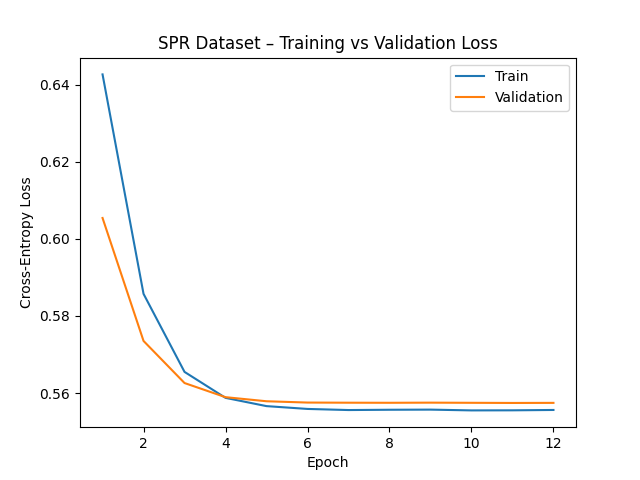
\includegraphics[width=\textwidth]{SPR_loss_curves.png}
        \caption{Training loss}
    \end{subfigure}
    \hfill
    \begin{subfigure}[b]{0.31\textwidth}
        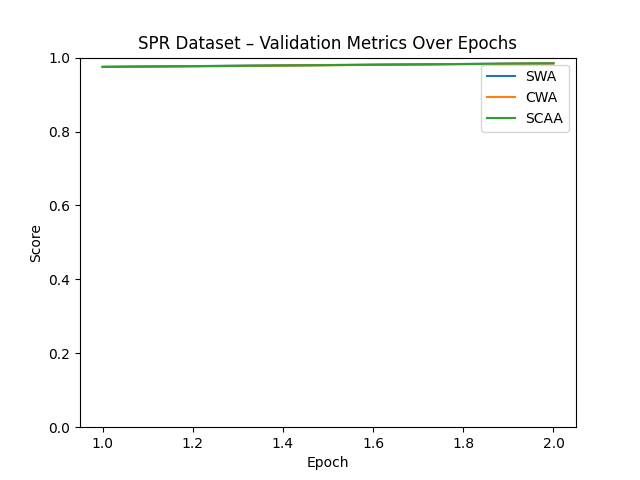
\includegraphics[width=\textwidth]{SPR_validation_metrics.png}
        \caption{Validation metrics}
    \end{subfigure}
    \hfill
    \begin{subfigure}[b]{0.31\textwidth}
        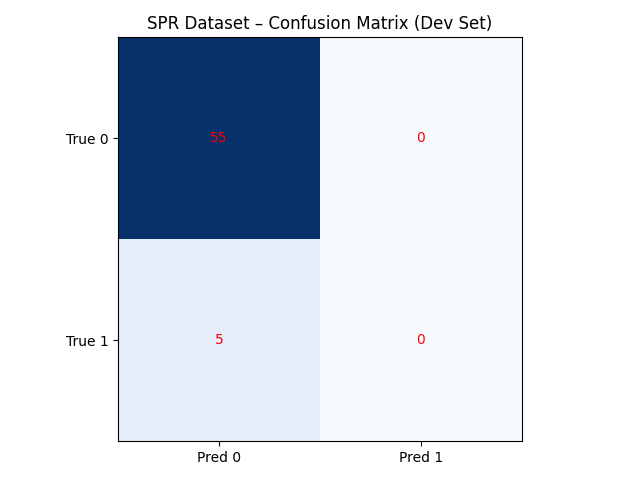
\includegraphics[width=\textwidth]{SPR_confusion_matrix.png}
        \caption{Confusion matrix}
    \end{subfigure}
    \caption{Core results. Symbolic proxies show early promise but fail to generalize: (a) training curves flatten quickly, (b) key metrics plateau, and (c) errors concentrate in overlapping categories.}
    \label{fig:combined}
\end{figure}

Additional figures illustrating alternative embeddings, per-seed runs, and ablation studies appear in the Appendix. Most of these confirm the same overall trend.

\section{Conclusion}
Our results expose pitfalls arising from the tension between symbolic proxies and continuous representations. Despite initial promise, the methods struggled with real-world shifts, highlighting the importance of transparent reporting and domain-focused validation. Future directions include hybridizing symbolic modules with robust uncertainty estimates to reduce these unexpected errors.

\clearpage
\bibliography{references}

\appendix

\section{Supplementary Materials}
Here, we include extended figures and details on hyperparameters, ablation studies, and domain-specific considerations. The supplementary plots provide single-seed breakdowns and additional confusion analyses to underscore the fragility under slight shifts in data distribution.

\end{document}